\documentclass[11pt]{article}
\usepackage[textwidth=18.0cm, textheight=23.0cm, top=2.0cm]{geometry}
\usepackage{pst-all}
\usepackage{amssymb}
\usepackage{tikz}
\usepackage{underscore}\begin{document}
\pagestyle{empty}


ClassName: \underline{\textbf{Class_03.2bp-34}}
\par
BinSize: \underline{\textbf{40 × 40}}
\par
ReduceSize: \underline{\textbf{40 × 40}}
\par
TypeNum: \underline{\textbf{77}}
\par
Num: \underline{\textbf{80}}
\par
OutS: \underline{\textbf{27200}}
\par
InS: \underline{\textbf{24958}}
\par
Rate: \underline{\textbf{0.918}}
\par
UB: \underline{\textbf{17}}
\par
LB0: \underline{\textbf{16}}
\par
LB: \underline{\textbf{17}}
\par
LBWithCut: \underline{\textbf{17}}
\par
NodeCut: \underline{\textbf{0}}
\par
ExtendedNodeCnt: \underline{\textbf{1}}
\par
GenNodeCnt: \underline{\textbf{1}}
\par
PrimalNode: \underline{\textbf{0}}
\par
ColumnCount: \underline{\textbf{288}}
\par
TotalCutCount: \underline{\textbf{0}}
\par
RootCutCount: \underline{\textbf{0}}
\par
LPSolverCnt: \underline{\textbf{272}}
\par
PricingSolverCnt: \underline{\textbf{272}}
\par
BranchAndBoundNum: \underline{\textbf{1}}
\par
isOpt: \underline{\textbf{true}}
\par
TimeOnInitSolution: \underline{\textbf{120.010 s}}
\par
TimeOnPrimal: \underline{\textbf{0.000 s}}
\par
TimeOnPricing: \underline{\textbf{562.436 s}}
\par
TimeOnRmp: \underline{\textbf{0.310 s}}
\par
TotalTime: \underline{\textbf{682.896 s}}
\par
\newpage


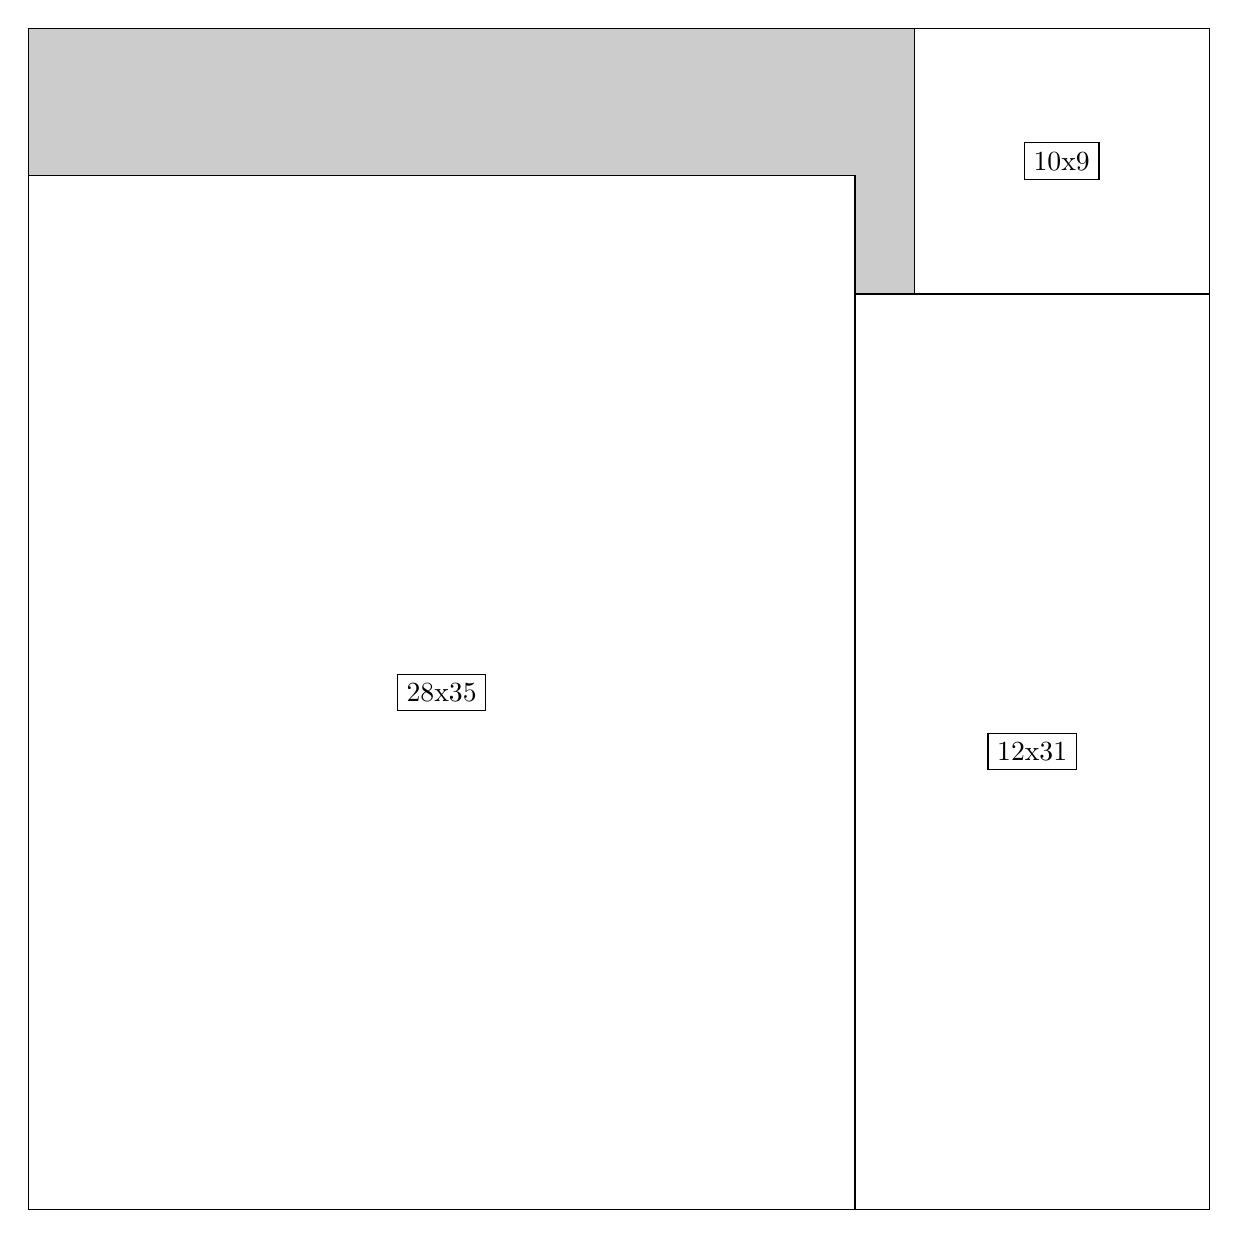
\begin{tikzpicture}[shorten >=1pt,scale=1.0,every node/.style={scale=1.0},->]
\tikzstyle{vertex}=[circle,fill=black!25,minimum size=14pt,inner sep=0pt]
\filldraw[fill=gray!40!white, draw=black] (0,0) rectangle (15.0,15.0);
\foreach \name/\x/\y/\w/\h in {28x35/0.0/0.0/10.5/13.125,12x31/10.5/0.0/4.5/11.625,10x9/11.25/11.625/3.75/3.375}
\filldraw[fill=white!40!white, draw=black] (\x,\y) rectangle node[draw] (\name) {\name} ++(\w,\h);
\end{tikzpicture}


w =28 , h =35 , x =0 , y =0 , v =980
\par
w =12 , h =31 , x =28 , y =0 , v =372
\par
w =10 , h =9 , x =30 , y =31 , v =90
\par
\newpage


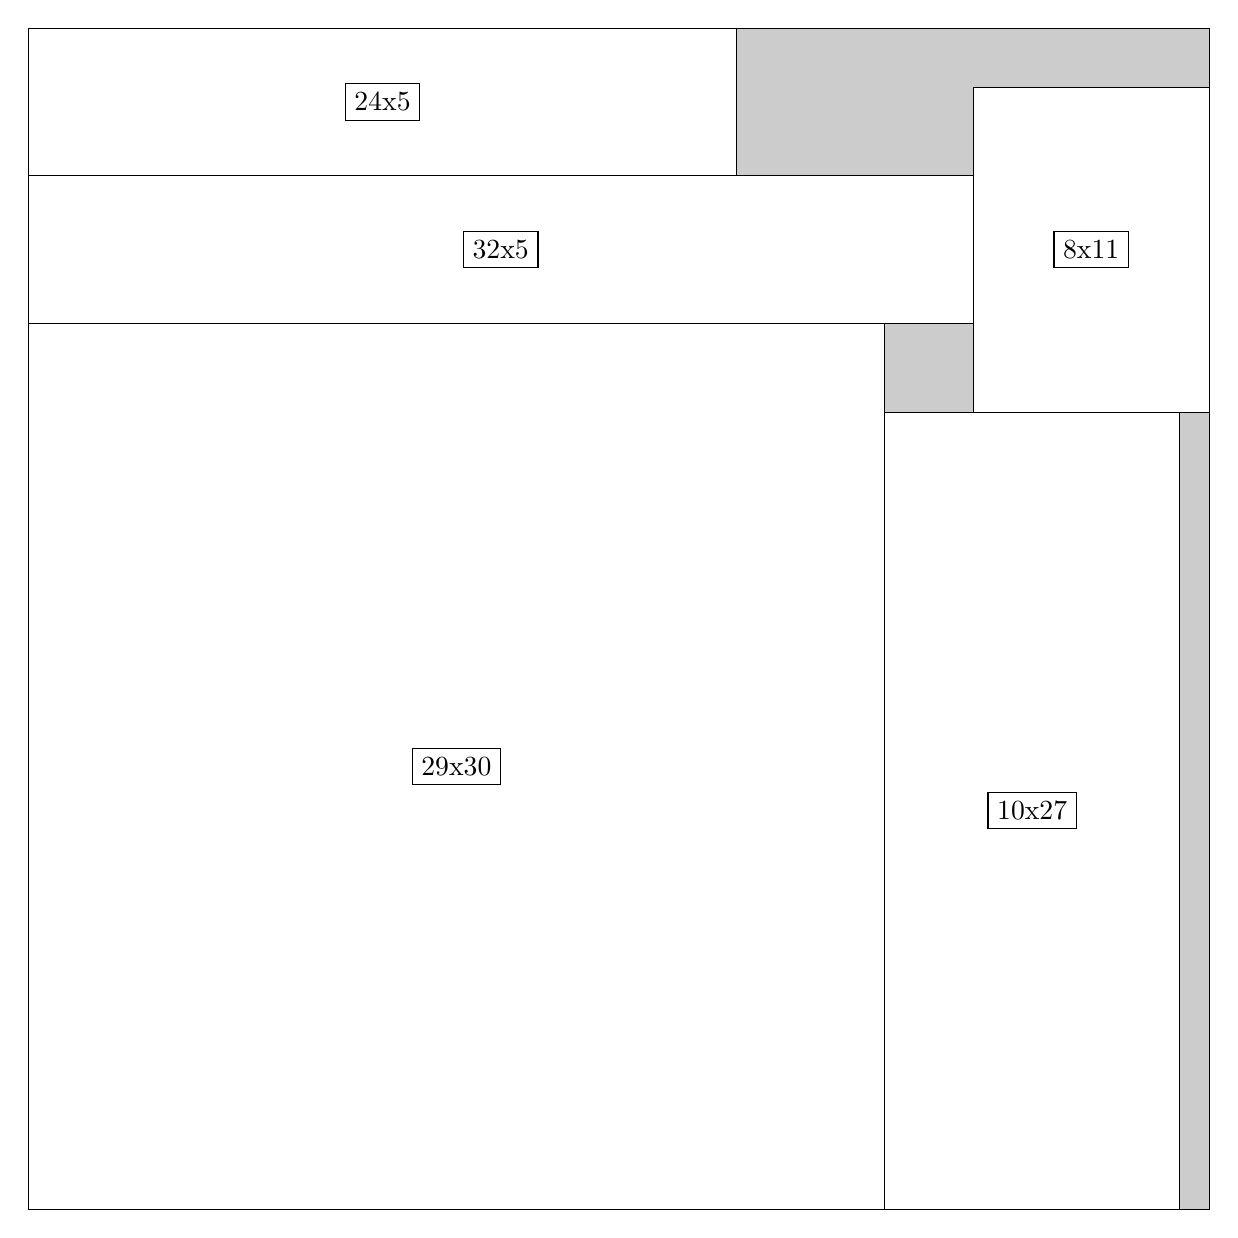
\begin{tikzpicture}[shorten >=1pt,scale=1.0,every node/.style={scale=1.0},->]
\tikzstyle{vertex}=[circle,fill=black!25,minimum size=14pt,inner sep=0pt]
\filldraw[fill=gray!40!white, draw=black] (0,0) rectangle (15.0,15.0);
\foreach \name/\x/\y/\w/\h in {29x30/0.0/0.0/10.875/11.25,10x27/10.875/0.0/3.75/10.125,32x5/0.0/11.25/12.0/1.875,24x5/0.0/13.125/9.0/1.875,8x11/12.0/10.125/3.0/4.125}
\filldraw[fill=white!40!white, draw=black] (\x,\y) rectangle node[draw] (\name) {\name} ++(\w,\h);
\end{tikzpicture}


w =29 , h =30 , x =0 , y =0 , v =870
\par
w =10 , h =27 , x =29 , y =0 , v =270
\par
w =32 , h =5 , x =0 , y =30 , v =160
\par
w =24 , h =5 , x =0 , y =35 , v =120
\par
w =8 , h =11 , x =32 , y =27 , v =88
\par
\newpage


\begin{tikzpicture}[shorten >=1pt,scale=1.0,every node/.style={scale=1.0},->]
\tikzstyle{vertex}=[circle,fill=black!25,minimum size=14pt,inner sep=0pt]
\filldraw[fill=gray!40!white, draw=black] (0,0) rectangle (15.0,15.0);
\foreach \name/\x/\y/\w/\h in {27x13/4.875/10.125/10.125/4.875,31x27/0.0/0.0/11.625/10.125,9x15/11.625/0.0/3.375/5.625,13x10/0.0/10.125/4.875/3.75,9x12/11.625/5.625/3.375/4.5,9x3/1.5/13.875/3.375/1.125}
\filldraw[fill=white!40!white, draw=black] (\x,\y) rectangle node[draw] (\name) {\name} ++(\w,\h);
\end{tikzpicture}


w =27 , h =13 , x =13 , y =27 , v =351
\par
w =31 , h =27 , x =0 , y =0 , v =837
\par
w =9 , h =15 , x =31 , y =0 , v =135
\par
w =13 , h =10 , x =0 , y =27 , v =130
\par
w =9 , h =12 , x =31 , y =15 , v =108
\par
w =9 , h =3 , x =4 , y =37 , v =27
\par
\newpage


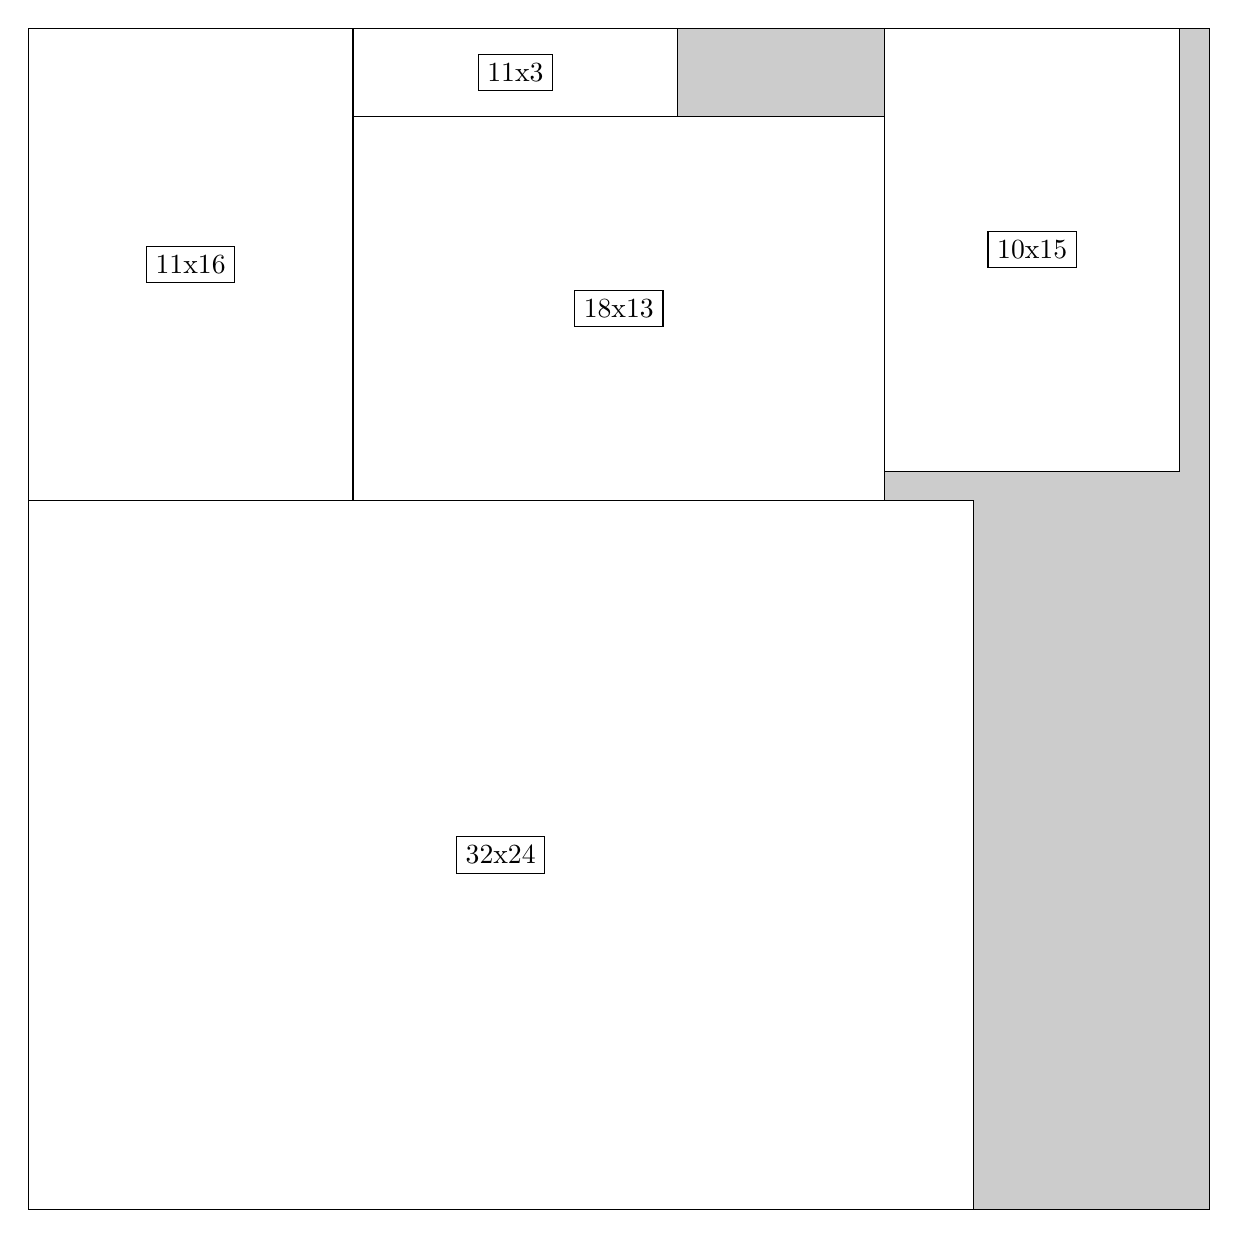
\begin{tikzpicture}[shorten >=1pt,scale=1.0,every node/.style={scale=1.0},->]
\tikzstyle{vertex}=[circle,fill=black!25,minimum size=14pt,inner sep=0pt]
\filldraw[fill=gray!40!white, draw=black] (0,0) rectangle (15.0,15.0);
\foreach \name/\x/\y/\w/\h in {32x24/0.0/0.0/12.0/9.0,18x13/4.125/9.0/6.75/4.875,11x16/0.0/9.0/4.125/6.0,10x15/10.875/9.375/3.75/5.625,11x3/4.125/13.875/4.125/1.125}
\filldraw[fill=white!40!white, draw=black] (\x,\y) rectangle node[draw] (\name) {\name} ++(\w,\h);
\end{tikzpicture}


w =32 , h =24 , x =0 , y =0 , v =768
\par
w =18 , h =13 , x =11 , y =24 , v =234
\par
w =11 , h =16 , x =0 , y =24 , v =176
\par
w =10 , h =15 , x =29 , y =25 , v =150
\par
w =11 , h =3 , x =11 , y =37 , v =33
\par
\newpage


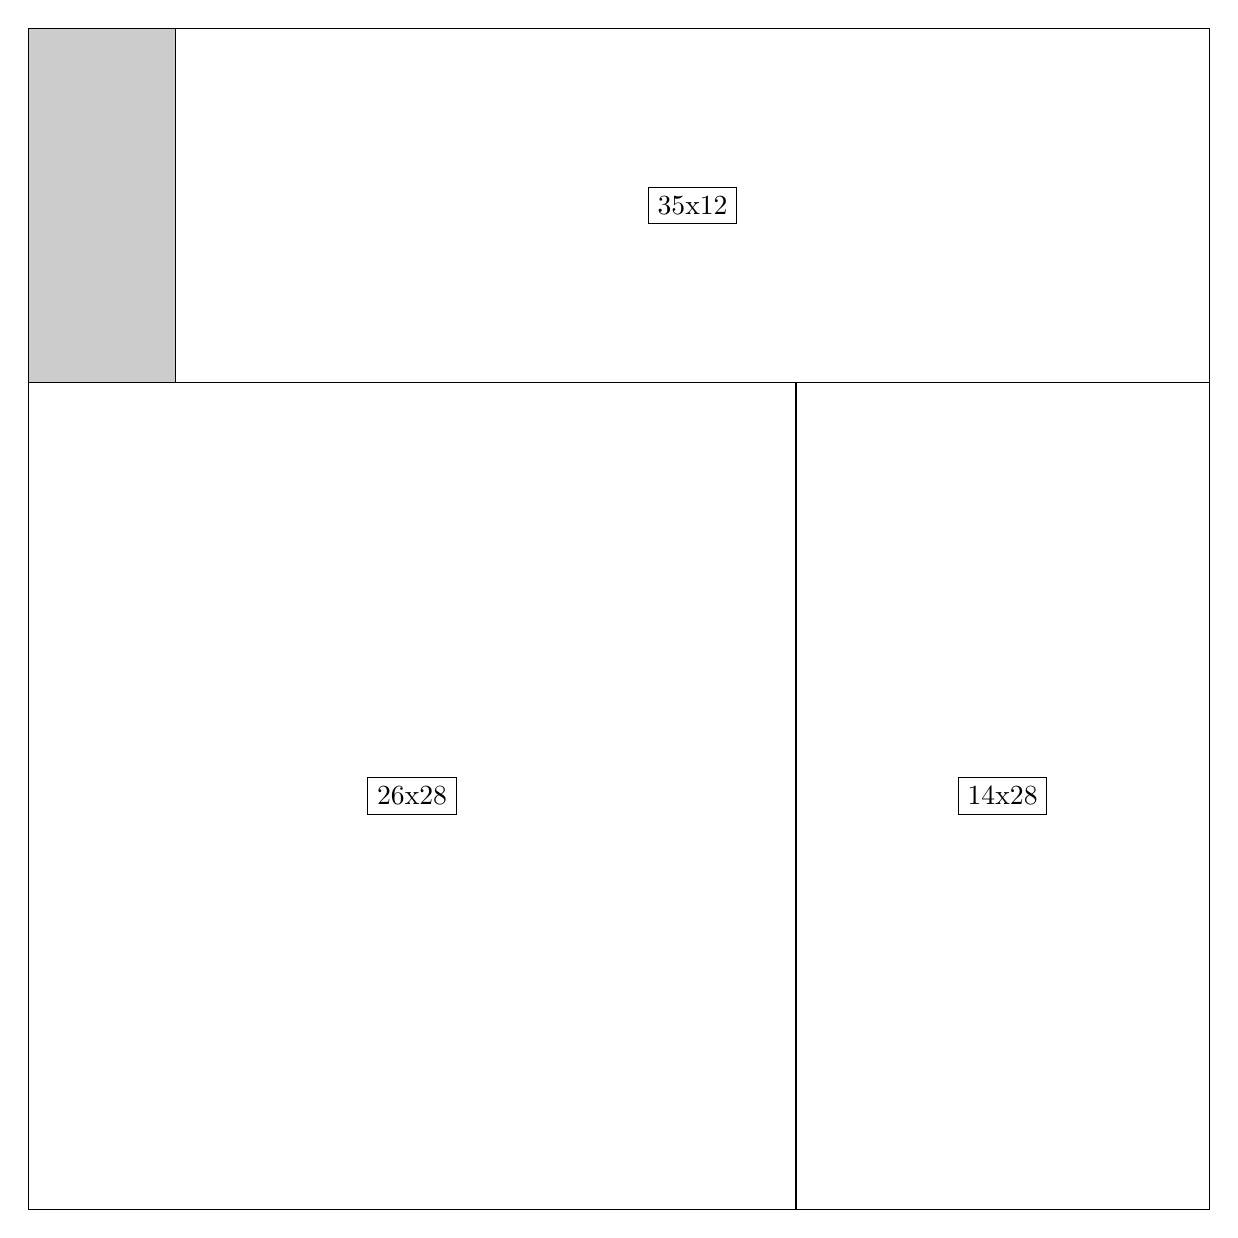
\begin{tikzpicture}[shorten >=1pt,scale=1.0,every node/.style={scale=1.0},->]
\tikzstyle{vertex}=[circle,fill=black!25,minimum size=14pt,inner sep=0pt]
\filldraw[fill=gray!40!white, draw=black] (0,0) rectangle (15.0,15.0);
\foreach \name/\x/\y/\w/\h in {26x28/0.0/0.0/9.75/10.5,35x12/1.875/10.5/13.125/4.5,14x28/9.75/0.0/5.25/10.5}
\filldraw[fill=white!40!white, draw=black] (\x,\y) rectangle node[draw] (\name) {\name} ++(\w,\h);
\end{tikzpicture}


w =26 , h =28 , x =0 , y =0 , v =728
\par
w =35 , h =12 , x =5 , y =28 , v =420
\par
w =14 , h =28 , x =26 , y =0 , v =392
\par
\newpage


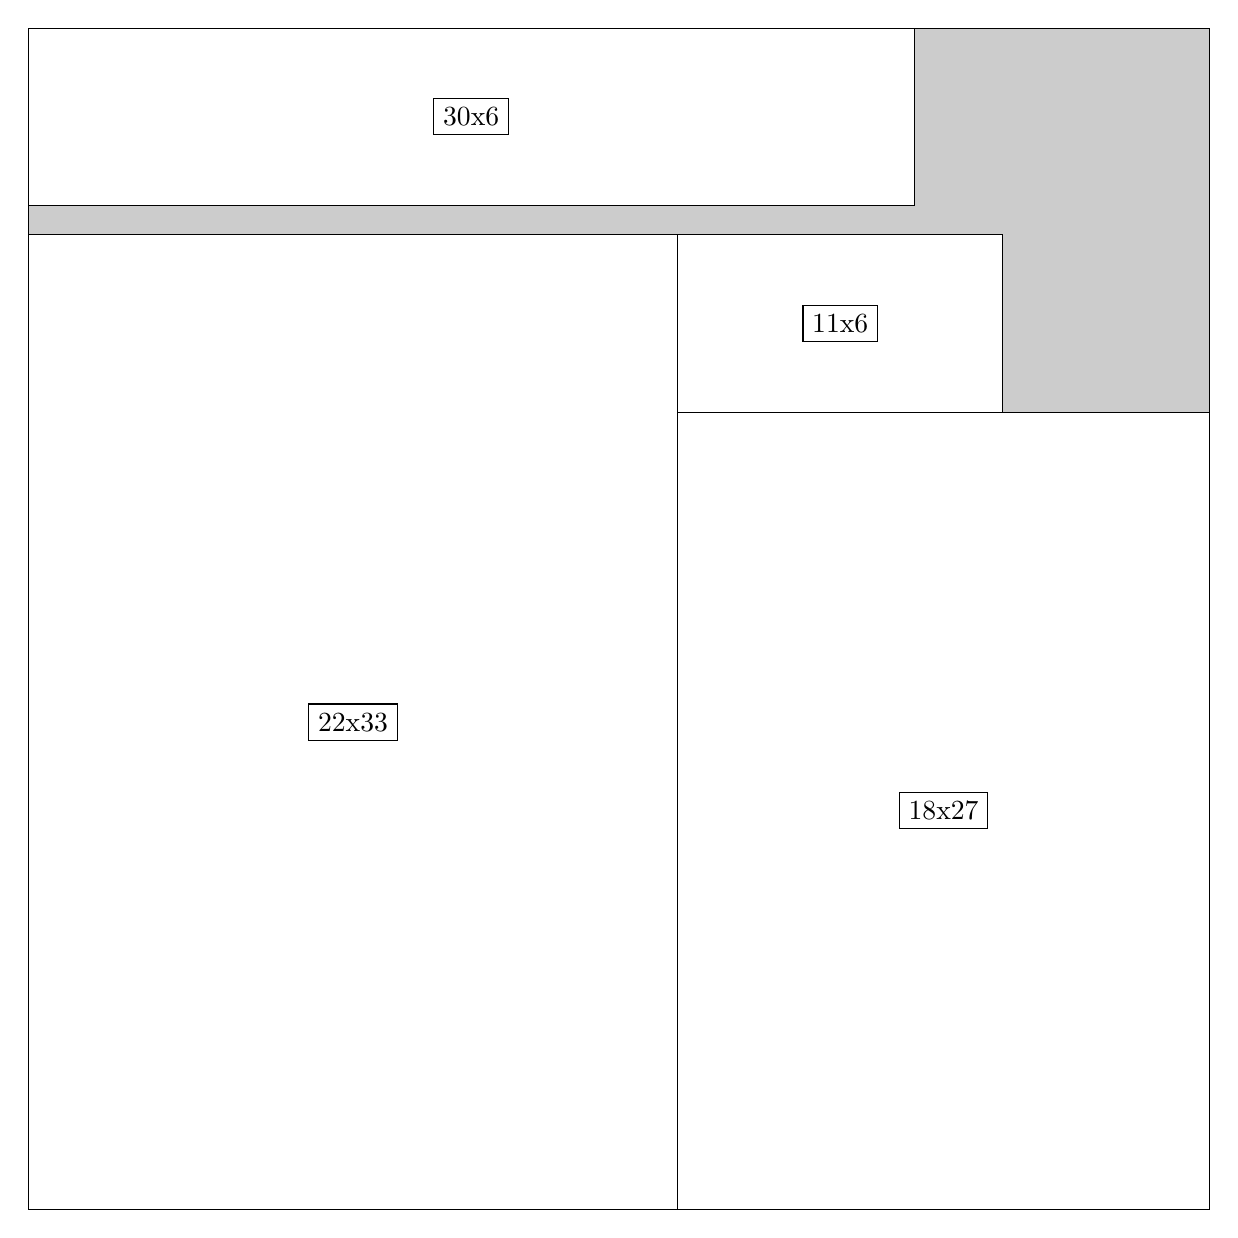
\begin{tikzpicture}[shorten >=1pt,scale=1.0,every node/.style={scale=1.0},->]
\tikzstyle{vertex}=[circle,fill=black!25,minimum size=14pt,inner sep=0pt]
\filldraw[fill=gray!40!white, draw=black] (0,0) rectangle (15.0,15.0);
\foreach \name/\x/\y/\w/\h in {22x33/0.0/0.0/8.25/12.375,18x27/8.25/0.0/6.75/10.125,30x6/0.0/12.75/11.25/2.25,11x6/8.25/10.125/4.125/2.25}
\filldraw[fill=white!40!white, draw=black] (\x,\y) rectangle node[draw] (\name) {\name} ++(\w,\h);
\end{tikzpicture}


w =22 , h =33 , x =0 , y =0 , v =726
\par
w =18 , h =27 , x =22 , y =0 , v =486
\par
w =30 , h =6 , x =0 , y =34 , v =180
\par
w =11 , h =6 , x =22 , y =27 , v =66
\par
\newpage


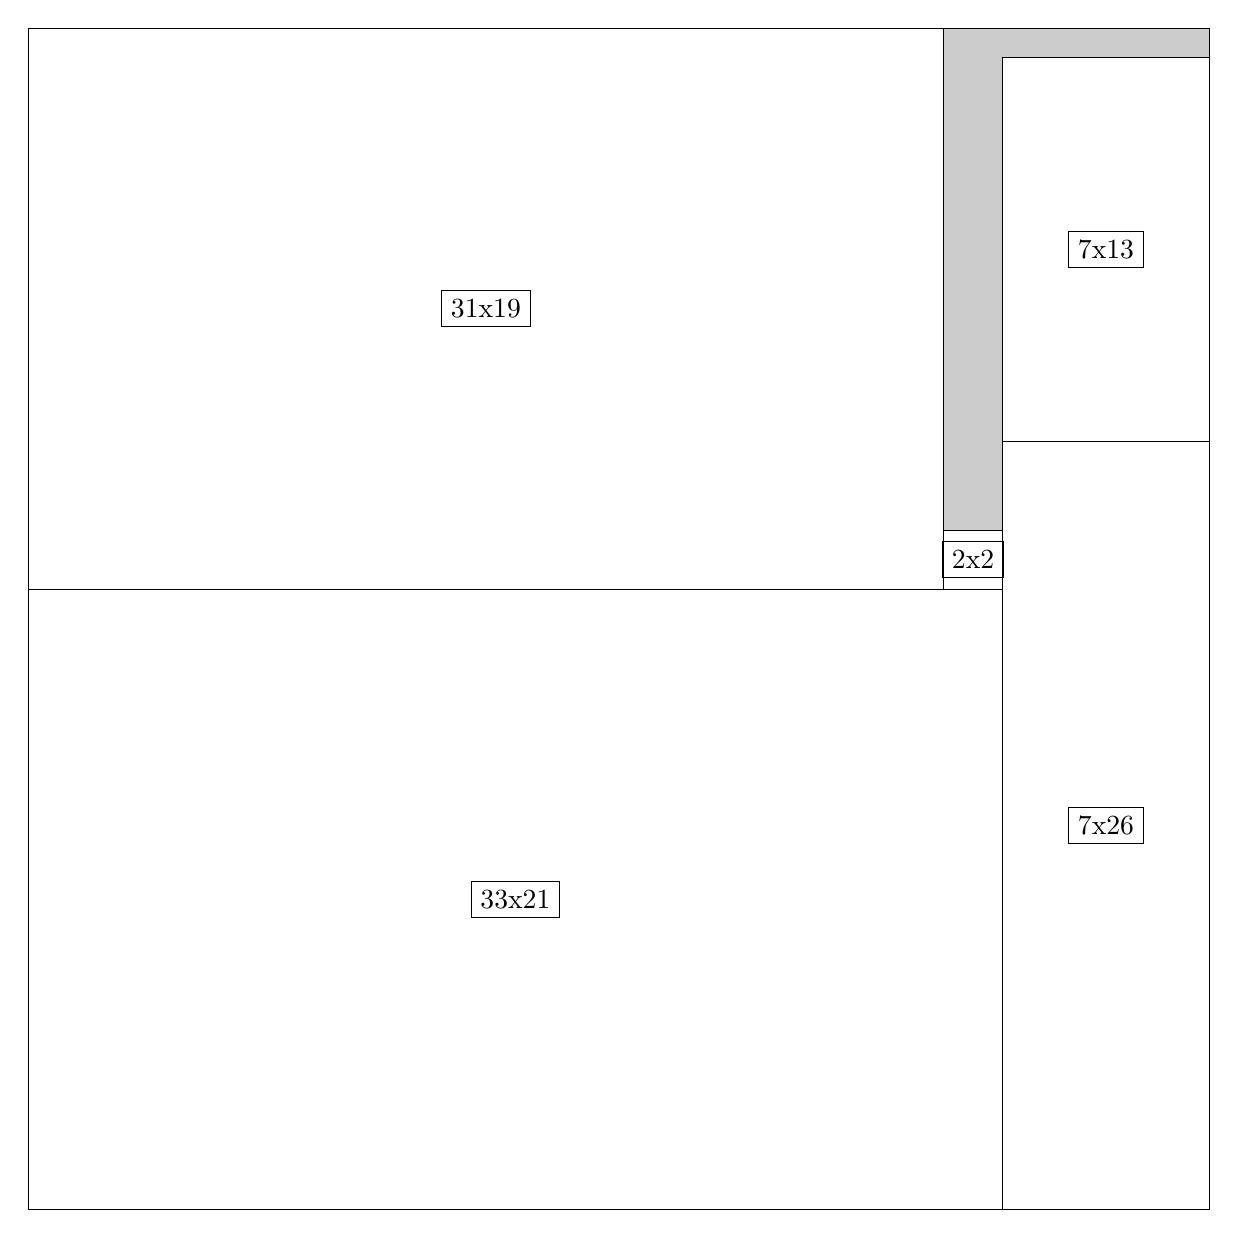
\begin{tikzpicture}[shorten >=1pt,scale=1.0,every node/.style={scale=1.0},->]
\tikzstyle{vertex}=[circle,fill=black!25,minimum size=14pt,inner sep=0pt]
\filldraw[fill=gray!40!white, draw=black] (0,0) rectangle (15.0,15.0);
\foreach \name/\x/\y/\w/\h in {33x21/0.0/0.0/12.375/7.875,31x19/0.0/7.875/11.625/7.125,7x26/12.375/0.0/2.625/9.75,7x13/12.375/9.75/2.625/4.875,2x2/11.625/7.875/0.75/0.75}
\filldraw[fill=white!40!white, draw=black] (\x,\y) rectangle node[draw] (\name) {\name} ++(\w,\h);
\end{tikzpicture}


w =33 , h =21 , x =0 , y =0 , v =693
\par
w =31 , h =19 , x =0 , y =21 , v =589
\par
w =7 , h =26 , x =33 , y =0 , v =182
\par
w =7 , h =13 , x =33 , y =26 , v =91
\par
w =2 , h =2 , x =31 , y =21 , v =4
\par
\newpage


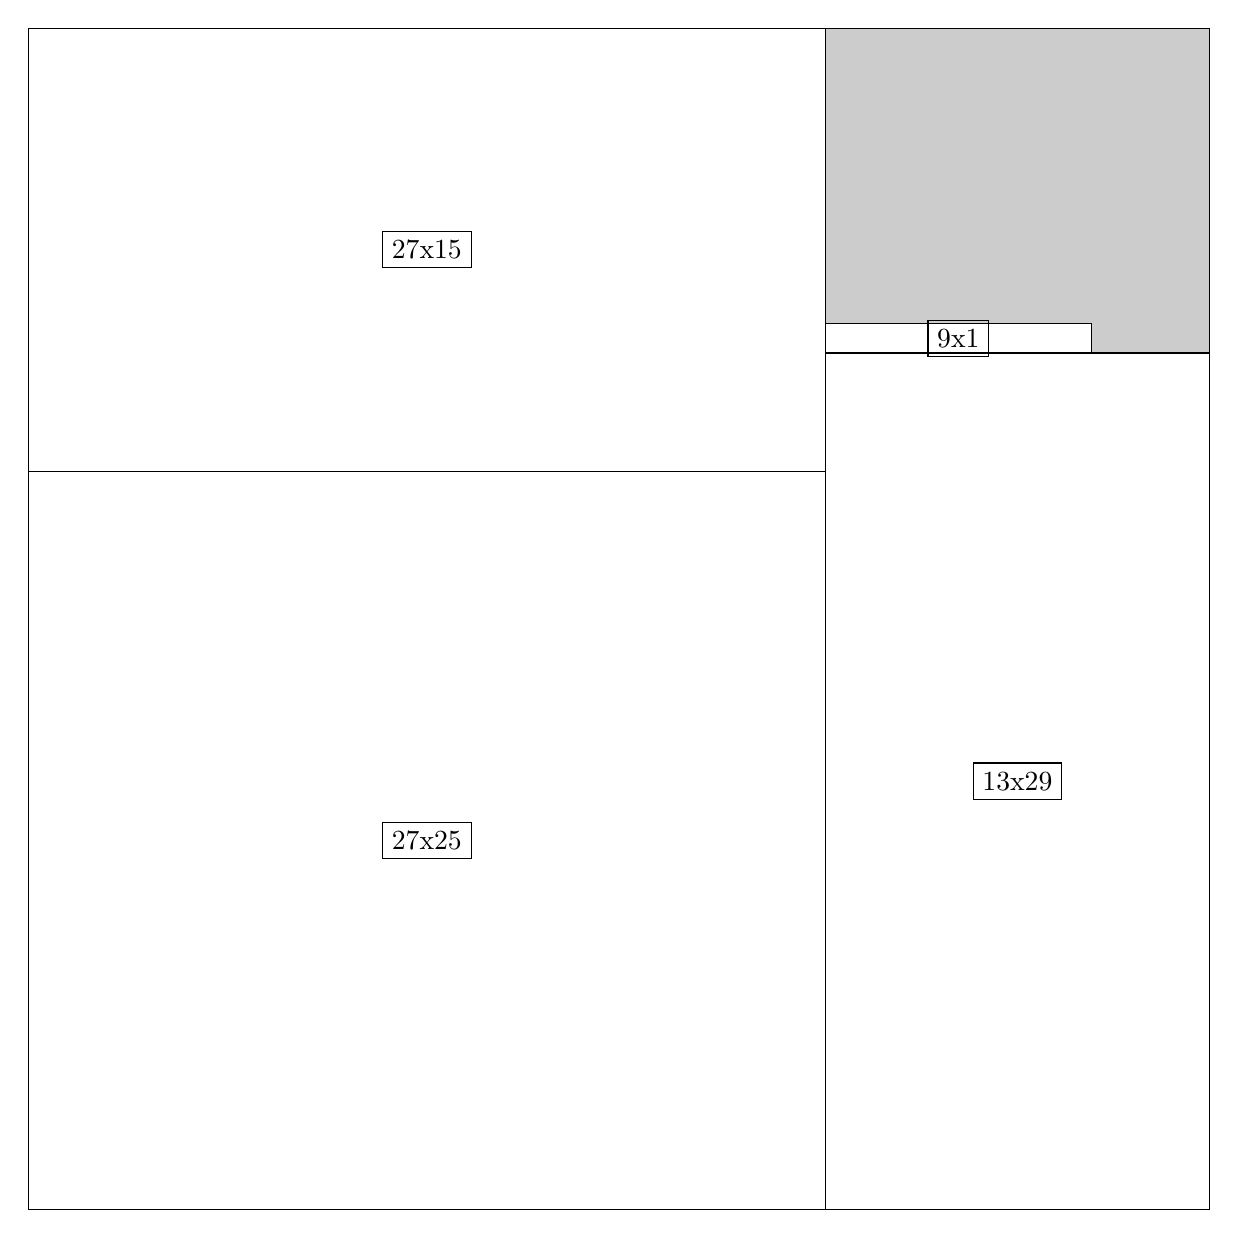
\begin{tikzpicture}[shorten >=1pt,scale=1.0,every node/.style={scale=1.0},->]
\tikzstyle{vertex}=[circle,fill=black!25,minimum size=14pt,inner sep=0pt]
\filldraw[fill=gray!40!white, draw=black] (0,0) rectangle (15.0,15.0);
\foreach \name/\x/\y/\w/\h in {27x15/0.0/9.375/10.125/5.625,13x29/10.125/0.0/4.875/10.875,27x25/0.0/0.0/10.125/9.375,9x1/10.125/10.875/3.375/0.375}
\filldraw[fill=white!40!white, draw=black] (\x,\y) rectangle node[draw] (\name) {\name} ++(\w,\h);
\end{tikzpicture}


w =27 , h =15 , x =0 , y =25 , v =405
\par
w =13 , h =29 , x =27 , y =0 , v =377
\par
w =27 , h =25 , x =0 , y =0 , v =675
\par
w =9 , h =1 , x =27 , y =29 , v =9
\par
\newpage


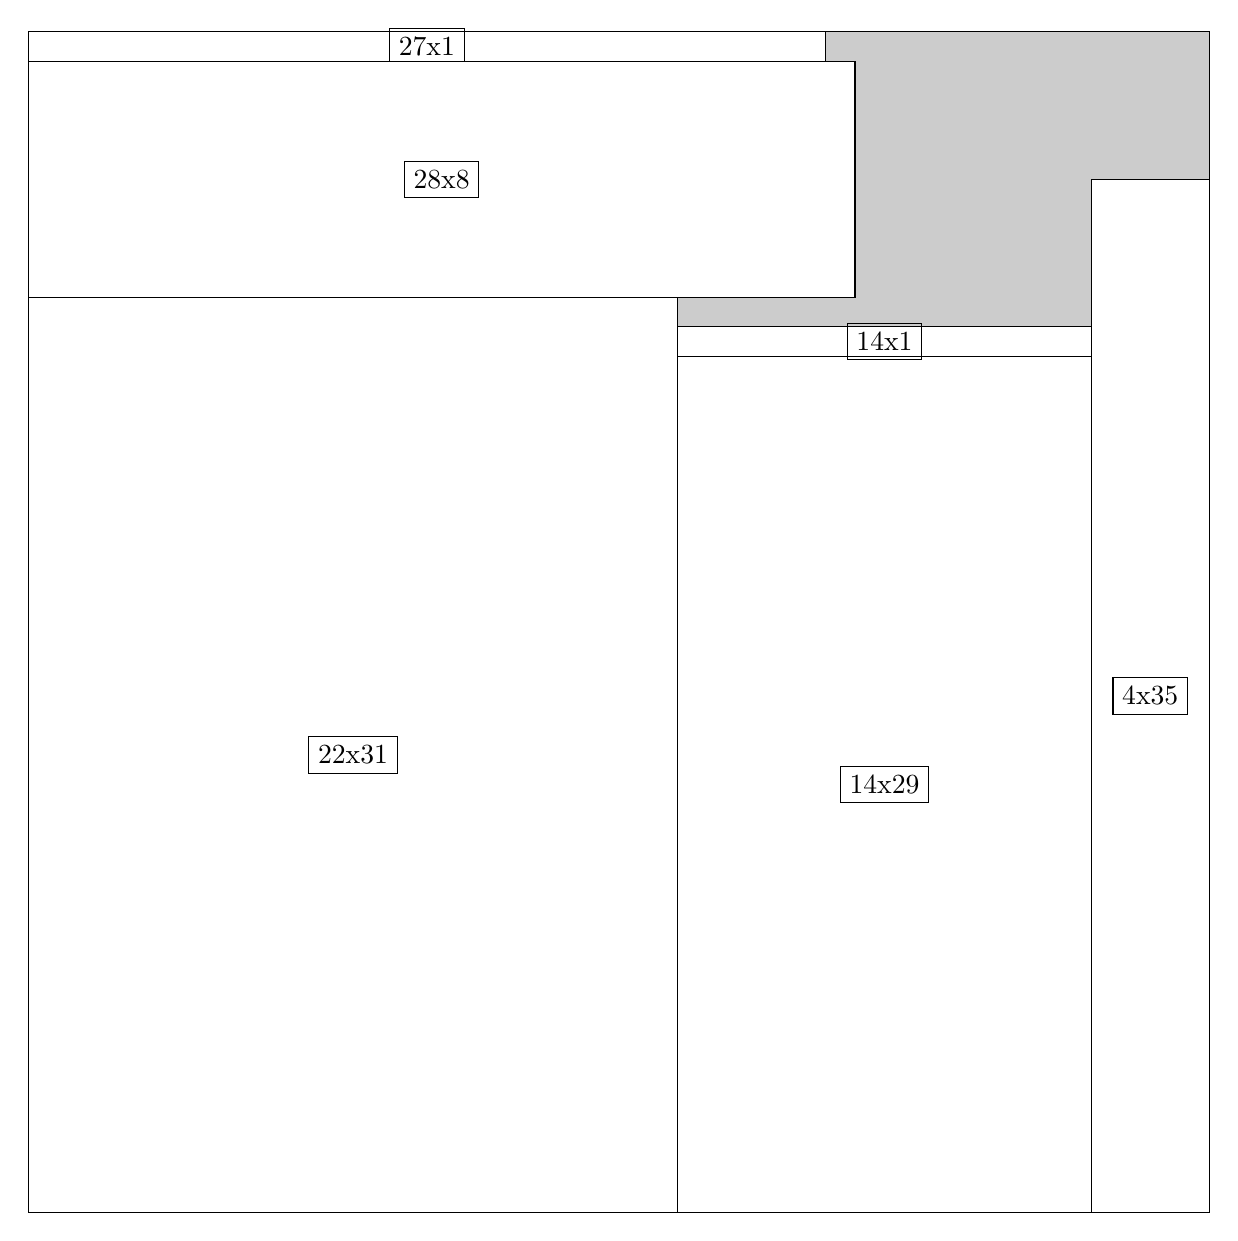
\begin{tikzpicture}[shorten >=1pt,scale=1.0,every node/.style={scale=1.0},->]
\tikzstyle{vertex}=[circle,fill=black!25,minimum size=14pt,inner sep=0pt]
\filldraw[fill=gray!40!white, draw=black] (0,0) rectangle (15.0,15.0);
\foreach \name/\x/\y/\w/\h in {22x31/0.0/0.0/8.25/11.625,27x1/0.0/14.625/10.125/0.375,28x8/0.0/11.625/10.5/3.0,4x35/13.5/0.0/1.5/13.125,14x29/8.25/0.0/5.25/10.875,14x1/8.25/10.875/5.25/0.375}
\filldraw[fill=white!40!white, draw=black] (\x,\y) rectangle node[draw] (\name) {\name} ++(\w,\h);
\end{tikzpicture}


w =22 , h =31 , x =0 , y =0 , v =682
\par
w =27 , h =1 , x =0 , y =39 , v =27
\par
w =28 , h =8 , x =0 , y =31 , v =224
\par
w =4 , h =35 , x =36 , y =0 , v =140
\par
w =14 , h =29 , x =22 , y =0 , v =406
\par
w =14 , h =1 , x =22 , y =29 , v =14
\par
\newpage


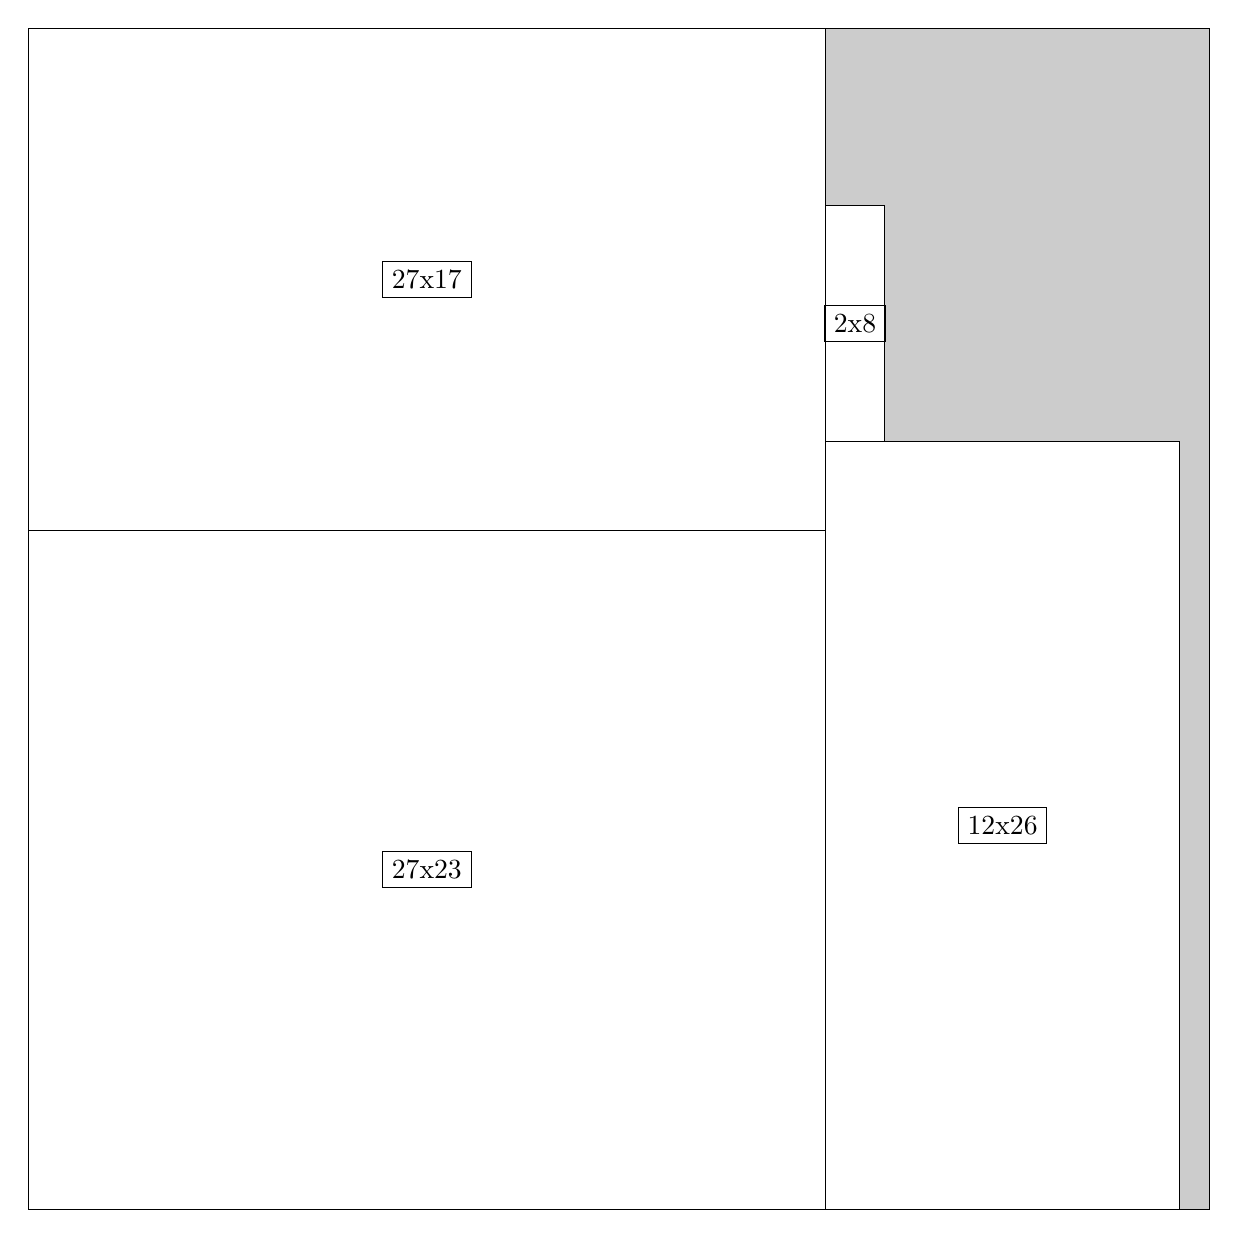
\begin{tikzpicture}[shorten >=1pt,scale=1.0,every node/.style={scale=1.0},->]
\tikzstyle{vertex}=[circle,fill=black!25,minimum size=14pt,inner sep=0pt]
\filldraw[fill=gray!40!white, draw=black] (0,0) rectangle (15.0,15.0);
\foreach \name/\x/\y/\w/\h in {27x23/0.0/0.0/10.125/8.625,27x17/0.0/8.625/10.125/6.375,12x26/10.125/0.0/4.5/9.75,2x8/10.125/9.75/0.75/3.0}
\filldraw[fill=white!40!white, draw=black] (\x,\y) rectangle node[draw] (\name) {\name} ++(\w,\h);
\end{tikzpicture}


w =27 , h =23 , x =0 , y =0 , v =621
\par
w =27 , h =17 , x =0 , y =23 , v =459
\par
w =12 , h =26 , x =27 , y =0 , v =312
\par
w =2 , h =8 , x =27 , y =26 , v =16
\par
\newpage


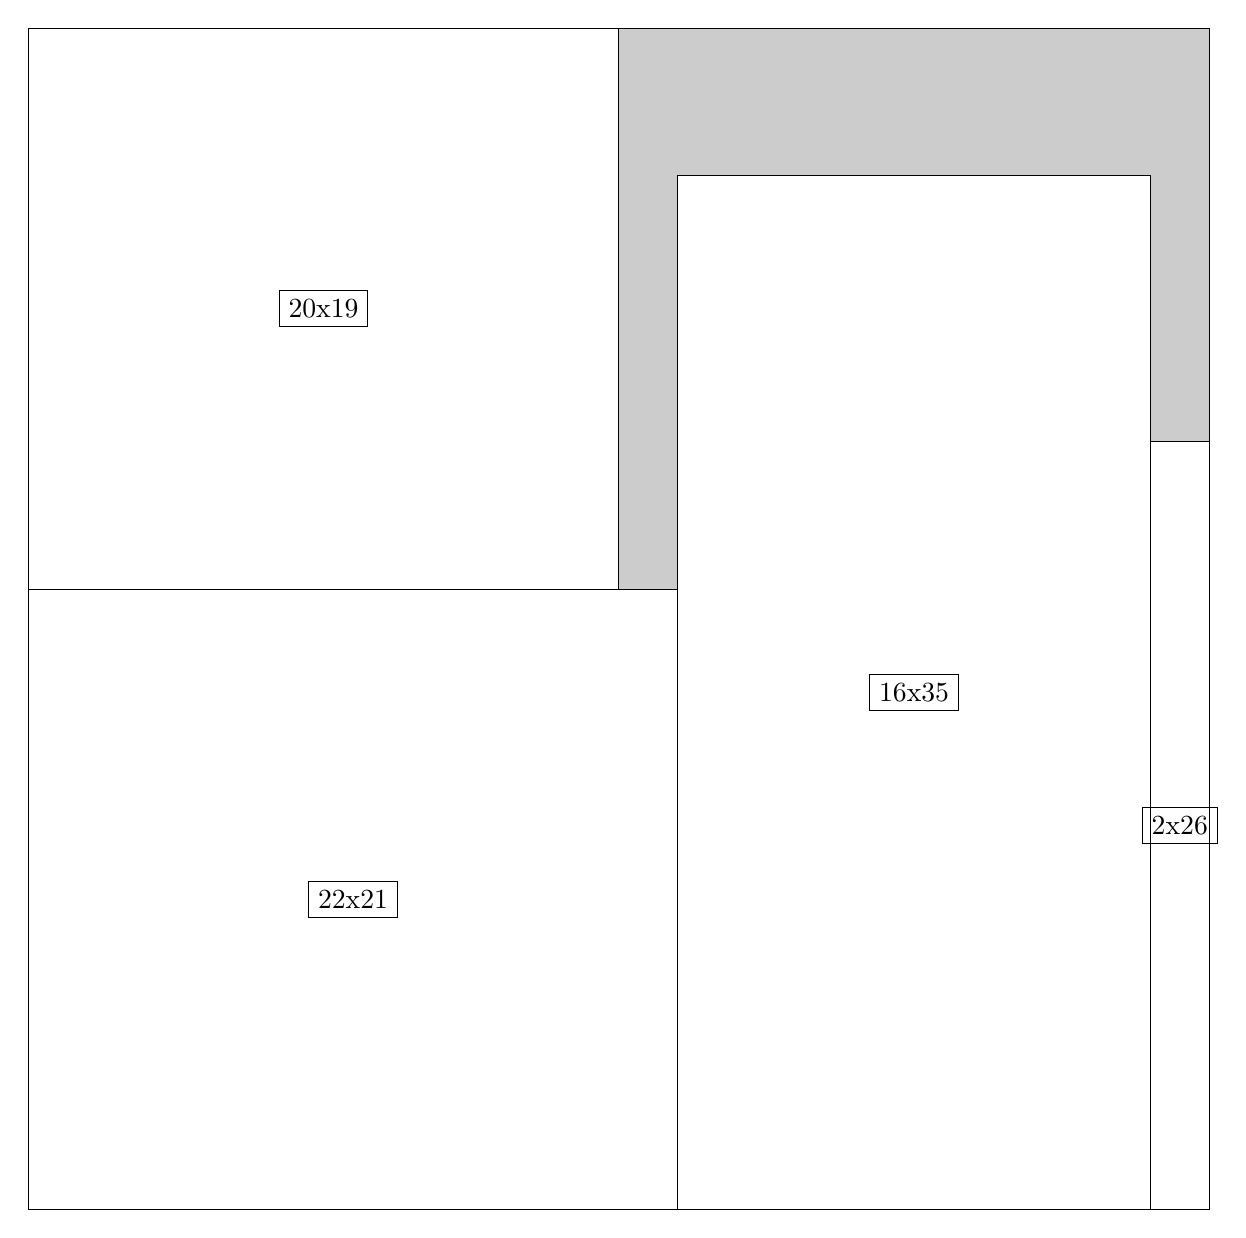
\begin{tikzpicture}[shorten >=1pt,scale=1.0,every node/.style={scale=1.0},->]
\tikzstyle{vertex}=[circle,fill=black!25,minimum size=14pt,inner sep=0pt]
\filldraw[fill=gray!40!white, draw=black] (0,0) rectangle (15.0,15.0);
\foreach \name/\x/\y/\w/\h in {16x35/8.25/0.0/6.0/13.125,22x21/0.0/0.0/8.25/7.875,20x19/0.0/7.875/7.5/7.125,2x26/14.25/0.0/0.75/9.75}
\filldraw[fill=white!40!white, draw=black] (\x,\y) rectangle node[draw] (\name) {\name} ++(\w,\h);
\end{tikzpicture}


w =16 , h =35 , x =22 , y =0 , v =560
\par
w =22 , h =21 , x =0 , y =0 , v =462
\par
w =20 , h =19 , x =0 , y =21 , v =380
\par
w =2 , h =26 , x =38 , y =0 , v =52
\par
\newpage


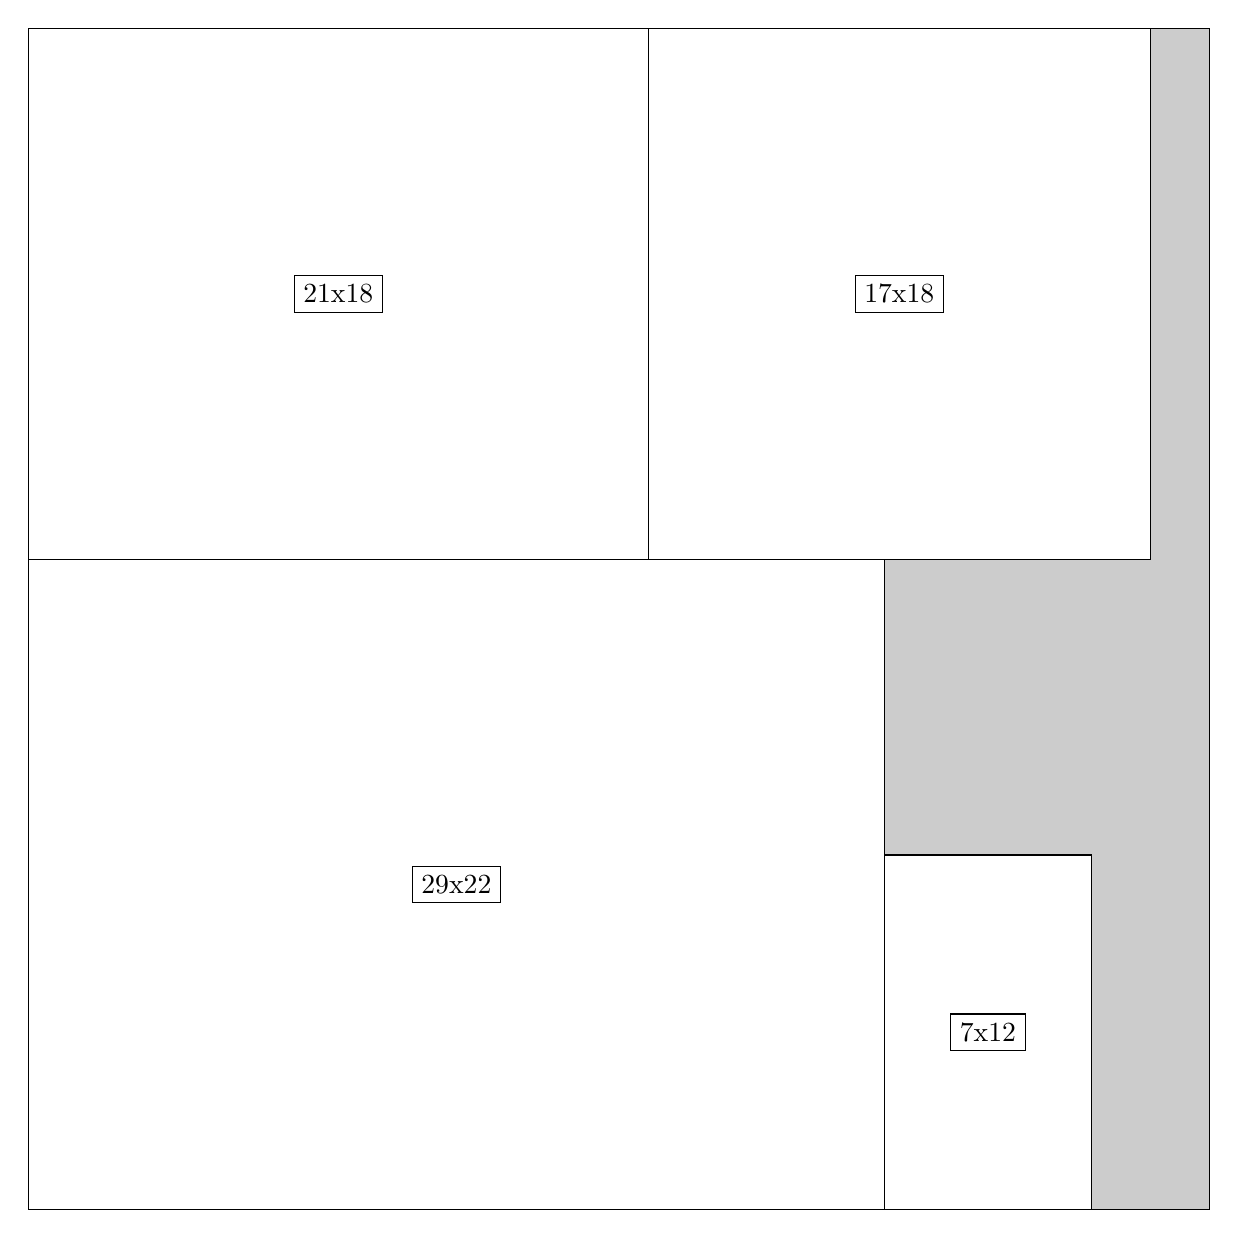
\begin{tikzpicture}[shorten >=1pt,scale=1.0,every node/.style={scale=1.0},->]
\tikzstyle{vertex}=[circle,fill=black!25,minimum size=14pt,inner sep=0pt]
\filldraw[fill=gray!40!white, draw=black] (0,0) rectangle (15.0,15.0);
\foreach \name/\x/\y/\w/\h in {29x22/0.0/0.0/10.875/8.25,21x18/0.0/8.25/7.875/6.75,17x18/7.875/8.25/6.375/6.75,7x12/10.875/0.0/2.625/4.5}
\filldraw[fill=white!40!white, draw=black] (\x,\y) rectangle node[draw] (\name) {\name} ++(\w,\h);
\end{tikzpicture}


w =29 , h =22 , x =0 , y =0 , v =638
\par
w =21 , h =18 , x =0 , y =22 , v =378
\par
w =17 , h =18 , x =21 , y =22 , v =306
\par
w =7 , h =12 , x =29 , y =0 , v =84
\par
\newpage


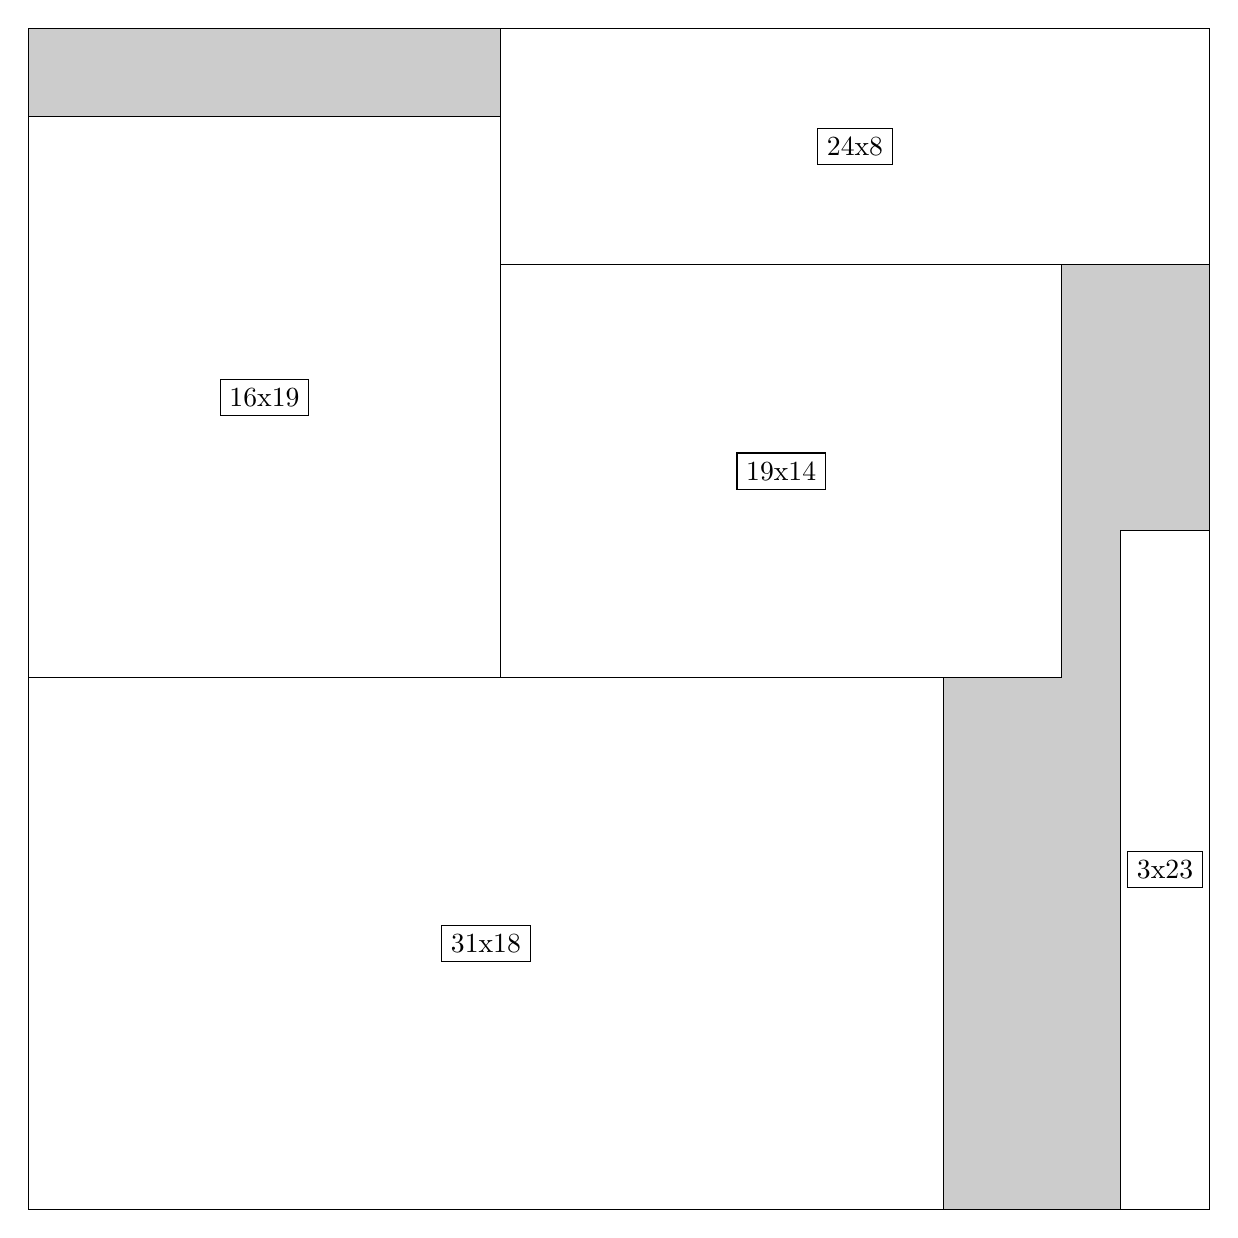
\begin{tikzpicture}[shorten >=1pt,scale=1.0,every node/.style={scale=1.0},->]
\tikzstyle{vertex}=[circle,fill=black!25,minimum size=14pt,inner sep=0pt]
\filldraw[fill=gray!40!white, draw=black] (0,0) rectangle (15.0,15.0);
\foreach \name/\x/\y/\w/\h in {31x18/0.0/0.0/11.625/6.75,3x23/13.875/0.0/1.125/8.625,16x19/0.0/6.75/6.0/7.125,19x14/6.0/6.75/7.125/5.25,24x8/6.0/12.0/9.0/3.0}
\filldraw[fill=white!40!white, draw=black] (\x,\y) rectangle node[draw] (\name) {\name} ++(\w,\h);
\end{tikzpicture}


w =31 , h =18 , x =0 , y =0 , v =558
\par
w =3 , h =23 , x =37 , y =0 , v =69
\par
w =16 , h =19 , x =0 , y =18 , v =304
\par
w =19 , h =14 , x =16 , y =18 , v =266
\par
w =24 , h =8 , x =16 , y =32 , v =192
\par
\newpage


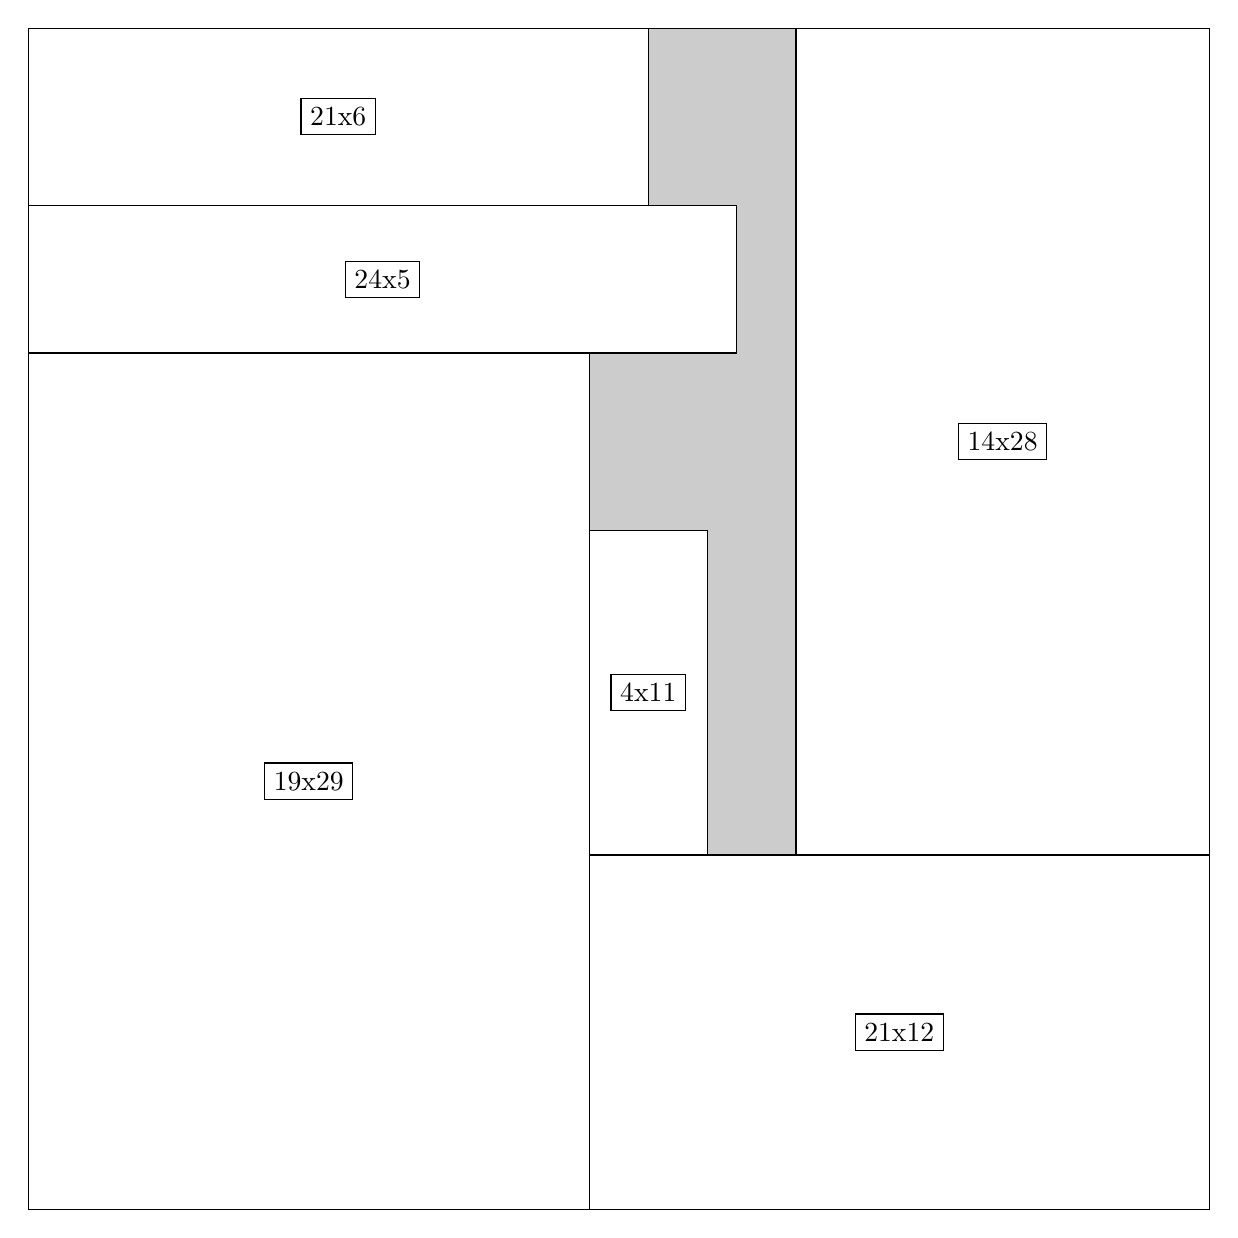
\begin{tikzpicture}[shorten >=1pt,scale=1.0,every node/.style={scale=1.0},->]
\tikzstyle{vertex}=[circle,fill=black!25,minimum size=14pt,inner sep=0pt]
\filldraw[fill=gray!40!white, draw=black] (0,0) rectangle (15.0,15.0);
\foreach \name/\x/\y/\w/\h in {19x29/0.0/0.0/7.125/10.875,14x28/9.75/4.5/5.25/10.5,21x12/7.125/0.0/7.875/4.5,21x6/0.0/12.75/7.875/2.25,24x5/0.0/10.875/9.0/1.875,4x11/7.125/4.5/1.5/4.125}
\filldraw[fill=white!40!white, draw=black] (\x,\y) rectangle node[draw] (\name) {\name} ++(\w,\h);
\end{tikzpicture}


w =19 , h =29 , x =0 , y =0 , v =551
\par
w =14 , h =28 , x =26 , y =12 , v =392
\par
w =21 , h =12 , x =19 , y =0 , v =252
\par
w =21 , h =6 , x =0 , y =34 , v =126
\par
w =24 , h =5 , x =0 , y =29 , v =120
\par
w =4 , h =11 , x =19 , y =12 , v =44
\par
\newpage


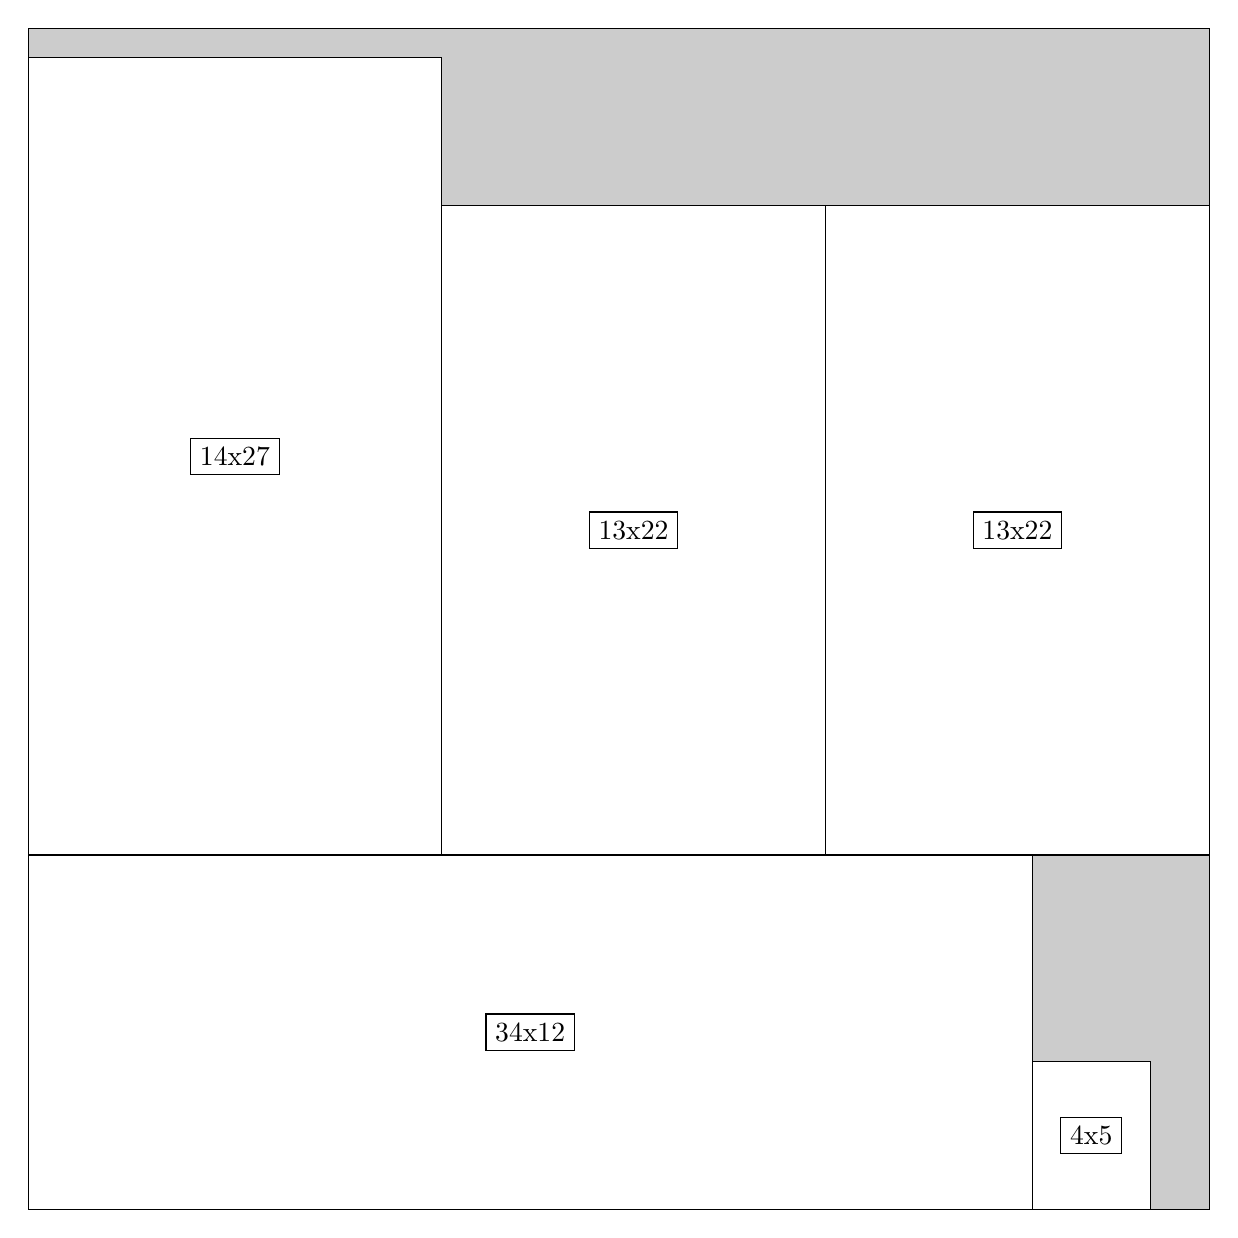
\begin{tikzpicture}[shorten >=1pt,scale=1.0,every node/.style={scale=1.0},->]
\tikzstyle{vertex}=[circle,fill=black!25,minimum size=14pt,inner sep=0pt]
\filldraw[fill=gray!40!white, draw=black] (0,0) rectangle (15.0,15.0);
\foreach \name/\x/\y/\w/\h in {34x12/0.0/0.0/12.75/4.5,14x27/0.0/4.5/5.25/10.125,13x22/5.25/4.5/4.875/8.25,13x22/10.125/4.5/4.875/8.25,4x5/12.75/0.0/1.5/1.875}
\filldraw[fill=white!40!white, draw=black] (\x,\y) rectangle node[draw] (\name) {\name} ++(\w,\h);
\end{tikzpicture}


w =34 , h =12 , x =0 , y =0 , v =408
\par
w =14 , h =27 , x =0 , y =12 , v =378
\par
w =13 , h =22 , x =14 , y =12 , v =286
\par
w =13 , h =22 , x =27 , y =12 , v =286
\par
w =4 , h =5 , x =34 , y =0 , v =20
\par
\newpage


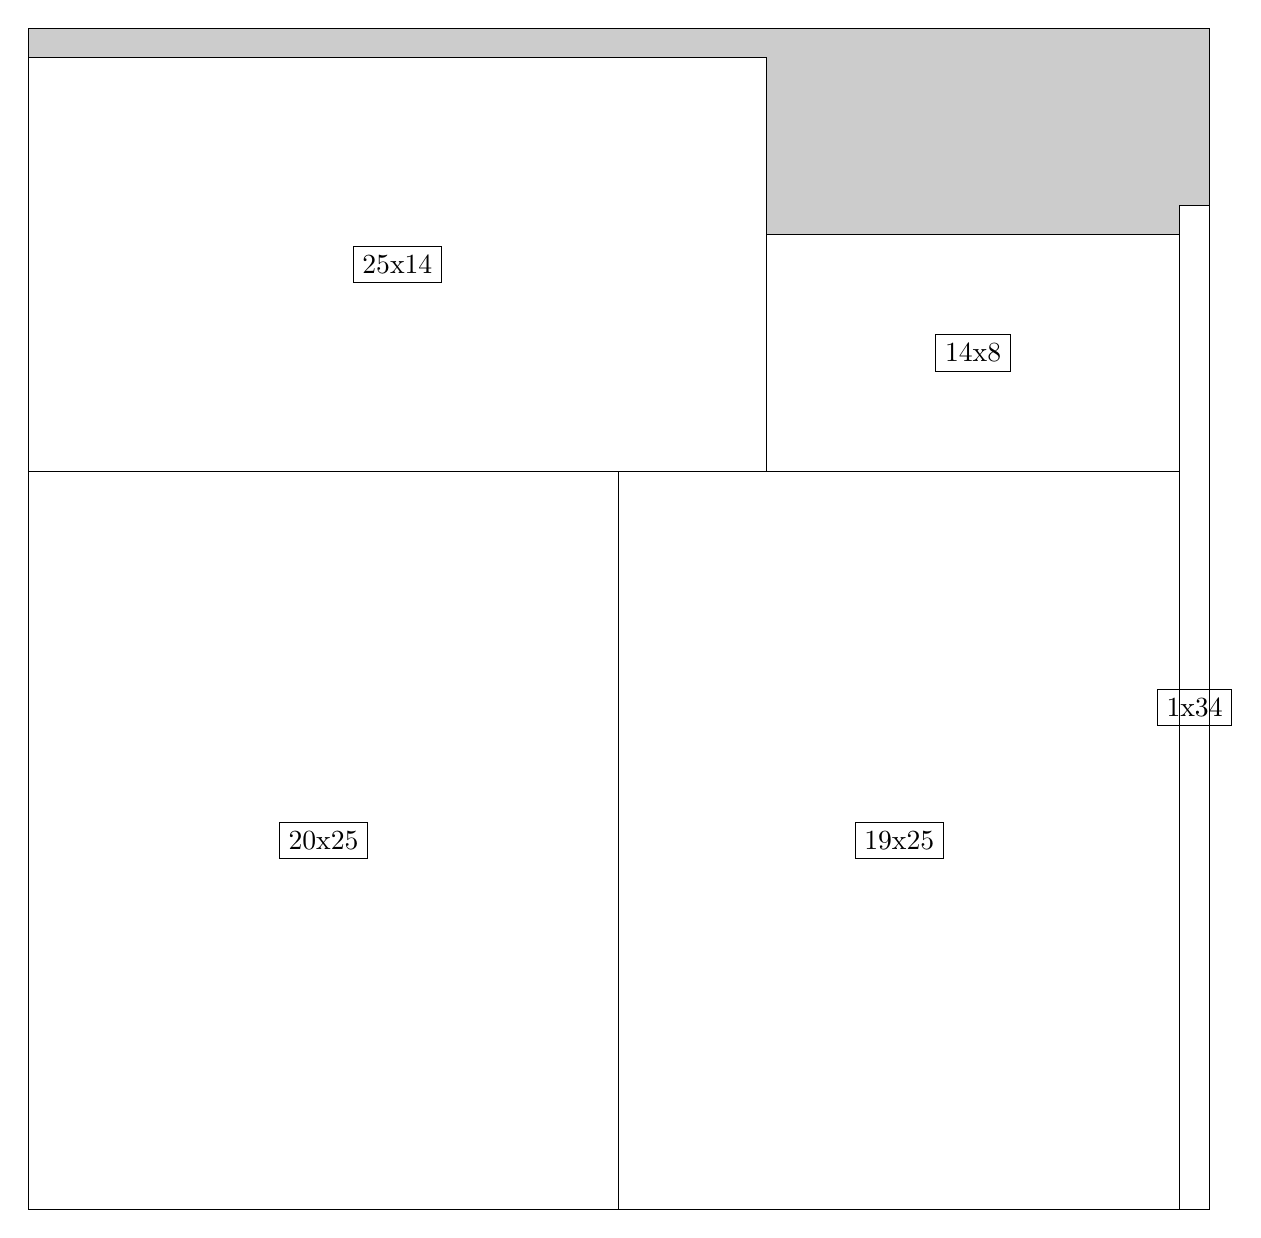
\begin{tikzpicture}[shorten >=1pt,scale=1.0,every node/.style={scale=1.0},->]
\tikzstyle{vertex}=[circle,fill=black!25,minimum size=14pt,inner sep=0pt]
\filldraw[fill=gray!40!white, draw=black] (0,0) rectangle (15.0,15.0);
\foreach \name/\x/\y/\w/\h in {20x25/0.0/0.0/7.5/9.375,19x25/7.5/0.0/7.125/9.375,25x14/0.0/9.375/9.375/5.25,14x8/9.375/9.375/5.25/3.0,1x34/14.625/0.0/0.375/12.75}
\filldraw[fill=white!40!white, draw=black] (\x,\y) rectangle node[draw] (\name) {\name} ++(\w,\h);
\end{tikzpicture}


w =20 , h =25 , x =0 , y =0 , v =500
\par
w =19 , h =25 , x =20 , y =0 , v =475
\par
w =25 , h =14 , x =0 , y =25 , v =350
\par
w =14 , h =8 , x =25 , y =25 , v =112
\par
w =1 , h =34 , x =39 , y =0 , v =34
\par
\newpage


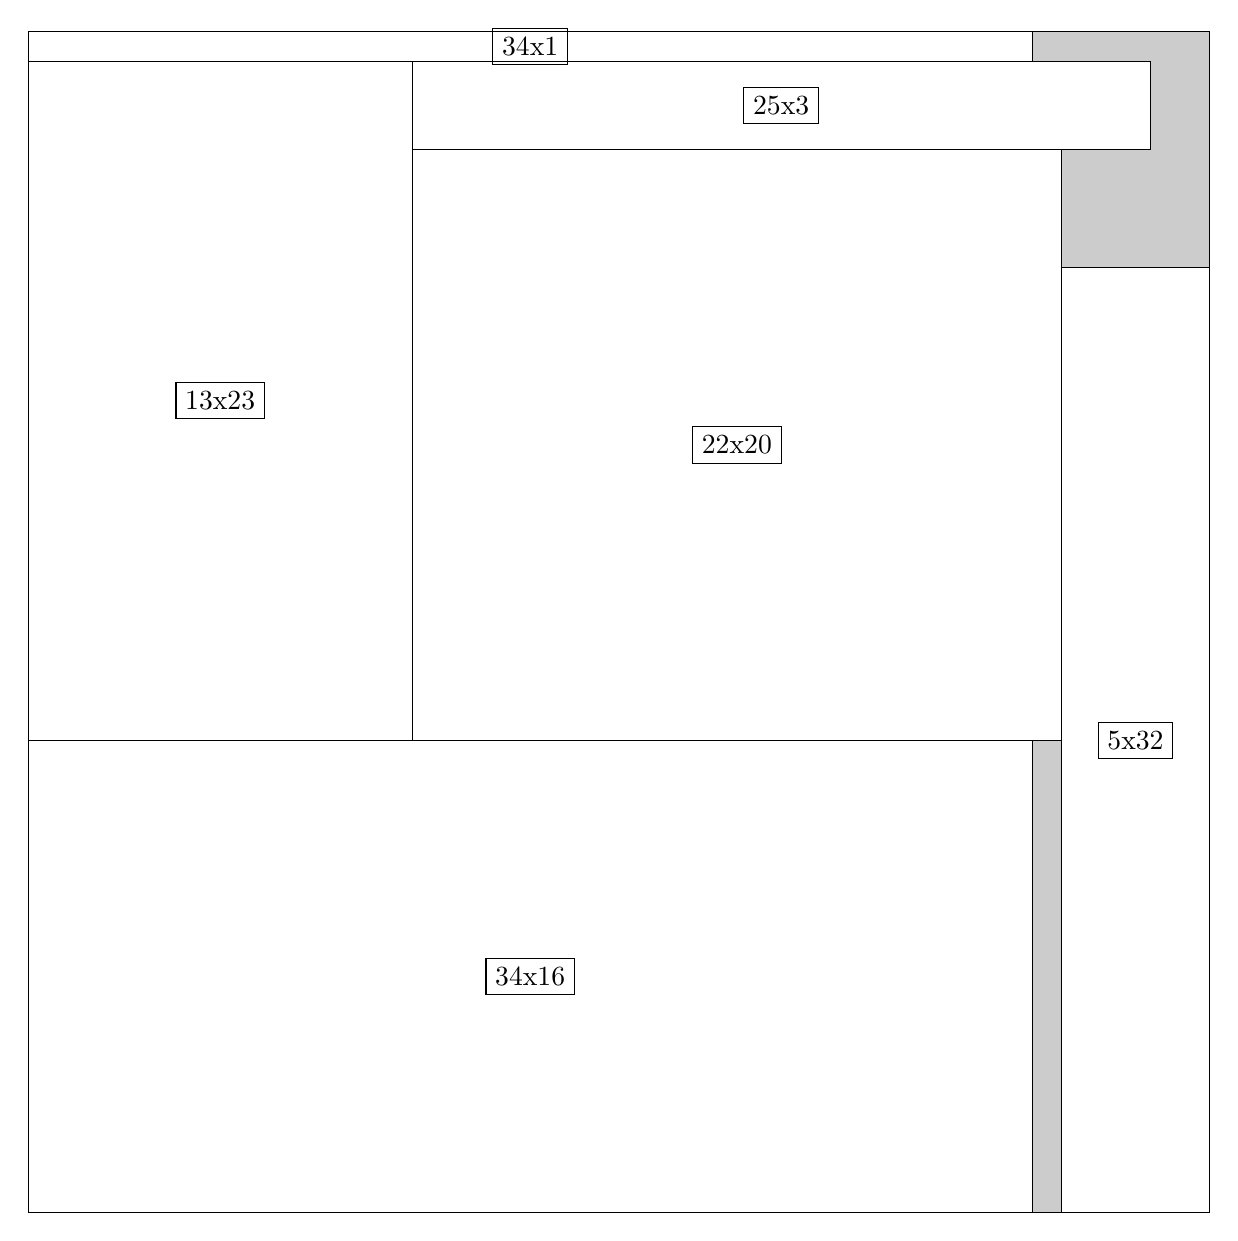
\begin{tikzpicture}[shorten >=1pt,scale=1.0,every node/.style={scale=1.0},->]
\tikzstyle{vertex}=[circle,fill=black!25,minimum size=14pt,inner sep=0pt]
\filldraw[fill=gray!40!white, draw=black] (0,0) rectangle (15.0,15.0);
\foreach \name/\x/\y/\w/\h in {34x16/0.0/0.0/12.75/6.0,13x23/0.0/6.0/4.875/8.625,5x32/13.125/0.0/1.875/12.0,25x3/4.875/13.5/9.375/1.125,22x20/4.875/6.0/8.25/7.5,34x1/0.0/14.625/12.75/0.375}
\filldraw[fill=white!40!white, draw=black] (\x,\y) rectangle node[draw] (\name) {\name} ++(\w,\h);
\end{tikzpicture}


w =34 , h =16 , x =0 , y =0 , v =544
\par
w =13 , h =23 , x =0 , y =16 , v =299
\par
w =5 , h =32 , x =35 , y =0 , v =160
\par
w =25 , h =3 , x =13 , y =36 , v =75
\par
w =22 , h =20 , x =13 , y =16 , v =440
\par
w =34 , h =1 , x =0 , y =39 , v =34
\par
\newpage


\end{document}